\section{Experimental Evaluation}
\label{sec:eval}

We obtained results through a process of collecting offline data, and modifying our simulator to output information about the data being processed. 
Mainly, we observed how changes in parameters affected the miss rate as well as the number of bytes transferred between the proxy and mobile device.

In order to run our experiments, we first collected offline data. 
Over the course of four days, we issued telnet GET requests to various webpages (both desktop and mobile versions) in the morning, afternoon and evening. 
The frequency with which we made these GET requests were for the purpose of reflecting browsing patterns, and it would give us information about the change in the content of a webpage over the course of a day and over the course of multiple days. 
We stored each response in a different file and then processed the data to obtain the byte stream version of the html pages. 
Using this byte stream, we ran several experiments that gave us insight into data redundancy within webpages.

Figure shows the distinctions between mobile web content and desktop web content. 
Many web servers today structure their webpages differently depending on the user-agent they're serving to increase the speed with which the webpages load, to provide better service with respect to UI and various other reasons. 
Therefore, mobile pages are inherently different from desktop browsers and thereby require its own analysis. 
Figure shows that the mobile version of cnn.com is only about a fifth of the size of the desktop version. 
The bytes transferred for the unchunked protocol shows that the size of the webpage remains relatively constant, and that the entire webpage has to be reloaded from the server for each request since the content is no longer "fresh". 
The bytes tranferred with the chunked protocol shows that the amount of redundancy that is eliminated in both mobile and desktop websites is proportional to the size of the web page. 
It also provides insight into exactly where our protocol performs well, and where the overhead of the protocol takes away from the benefits achieved from chunking. 
We see that on the first visit, the amount of bytes that needs to be transferred is almost twice the size of the actual content. 
This inefficiency comes from the fact that we're using chunk size of ten bytes. 
During the first visit to cnn.com, when there is no base copy of the webpage, the fingerprints representing the entire webpage need to be sent back and forth creating an inefficiency. 
However, once there is a base copy in the cache, the overhead decreases substantially. 
We can see from the graph that by the 12th visit, we are only transferring half the number of bytes as we would need to reload the entire webpage. 

The use of chunk size of 10 bytes means that each redundant chunk saves 6 bytes because of the 4 bytes of fingerprint needed to represent that chunk. 
This led us to explore different chunksizes to find the ideal chunk size that takes into consideration the tradeoff between having a low cache miss rate and having a fingerprint map to a bigger chunk. 
This is innately tied to the size of the content. Figure shows the relationship between \% of web content that is needed (based on cache miss rate) and chunk size based on a series of visits to cnn.com. 
The first visit is not shown since the cache is empty and so 100\% of the content needs to be transferred for all chunk sizes. 
The graph shows data from the second day, assuming cache has already been filled with data from the first visit. 
It is clear from this graph that if we use smaller chunk sizes, the percent of content that needs to be sent decreases. 
The steeper line for chunk 5 when compared to chunk 45 shows that as the number of visits increase, the overlap of smaller chunk sizes increases faster.
However, it means that each fingerprint maps to a smaller chunk and so more fingerprints are needed to represent the small amount of data that needs to be transferred and fewer fingerprints are needed to represent a large amount of data. 
In figure we can see that as the chunk size increased, the miss rate also increased as expected, but the bytes transferred actually decreased. 
This is because if the chunk size is small it gets expensive for the mobile device to communicate which chunks it needs. 
At this point, the ideal chunk size depends on the size of content that needs to be transferred as opposed to percentage.

The next two graphs show what happens when we visisted three websites three times a day for four days to simulate "mobile browsing". 
Figure shows that on the the first visit, the cache is empty and 100\% of the traffic needs to be transferred. 
For the second website, almost all of it needs to be transferred (~90\%) because of lack of overlap with the first website. 
On the third, the proportion decreases further but a majority of the page still needs to be transferred. 
After this point, we have the base page for all three websites in our cache and only the differences need to be transferred from the proxy, so the proportion of content that needs to be transferred stays below 20\% by the sixth url request. 
This figure calculates the proportion of content that needs to be transferred based on the cache miss rate but does not take into account the additional bytes that have to be transferred due to fingerprints.

Figure shows the total number of bytes that were transferred for the 32 requests. 
We assume that no response is identical to a previous response. 
This means that without chunking, the full webpage has to be reloaded for each request, leading to the linearly increasing number of bytes we see in the graph. 
With chunking however, we see that past the first few requests in which the effects of the overhead are heavy, the number of total bytes transferred rises gradually, and the gap between the bytes transferred grows with the number of requests.


\begin{figure}[h] 
\centering 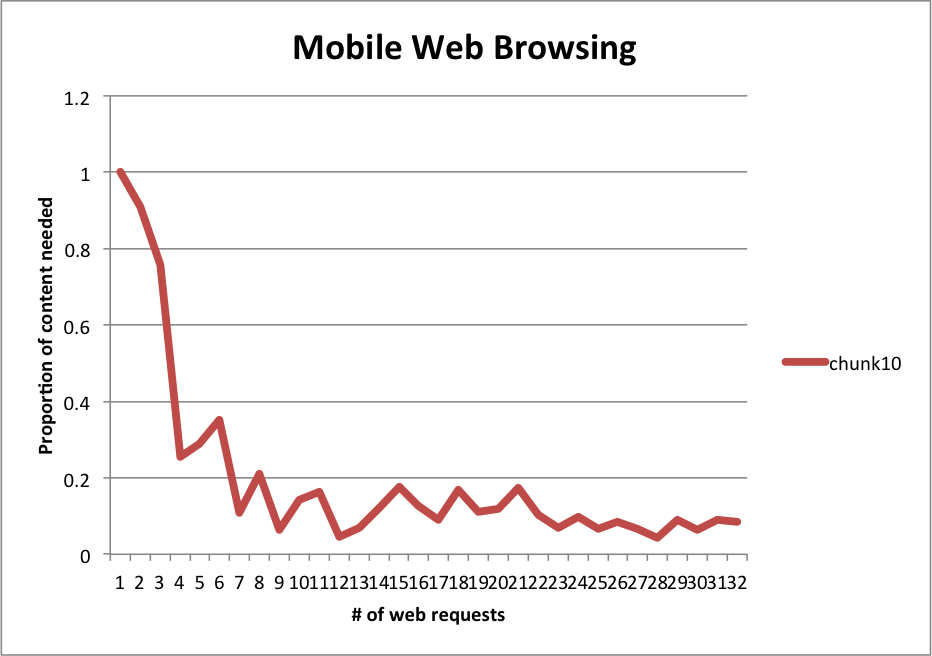
\includegraphics[scale=0.40]{images/browsing.png}
\caption{Mobile Web Browsing. The data was gathered by visiting cnn.com, nytimes.com and economist.com in an alternating basis three times a day over four days. This graph shows that the if the 'base' content of each webpage is in the cache, then less than 20\% of the content is generally new. The first three requests show that there is some, but not a lot of redundancy between webpages.}
\end{figure}

\begin{figure}[h] 
\centering 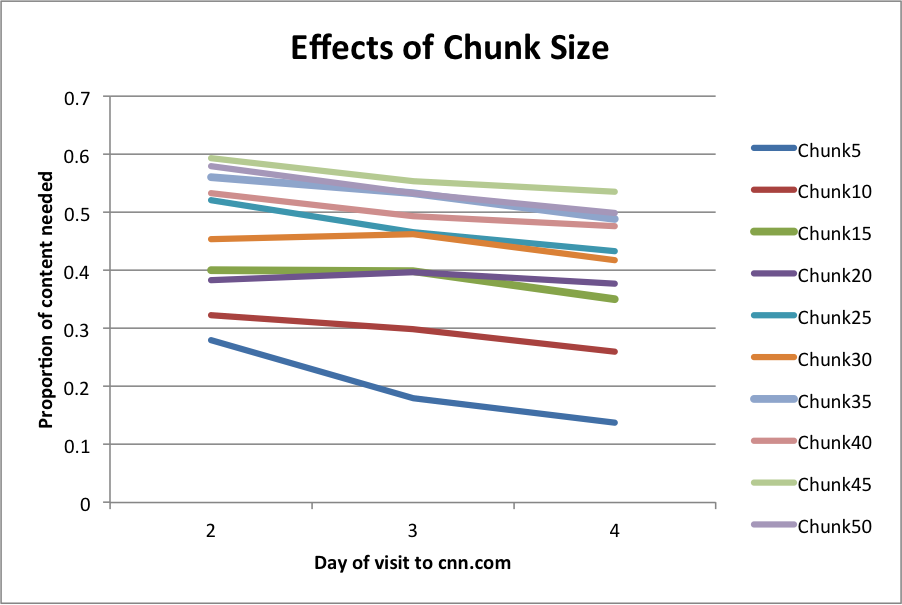
\includegraphics[scale=0.40]{images/chunksize.png}
\caption{Effects of Chunk Size on portion of content needed obtained through visit to cnn once a day for four days. Day 1 is not shown since the cache is empty so the contents of the entire webpage needs to be transferred.}
\end{figure}

\begin{figure}[h] 
\centering 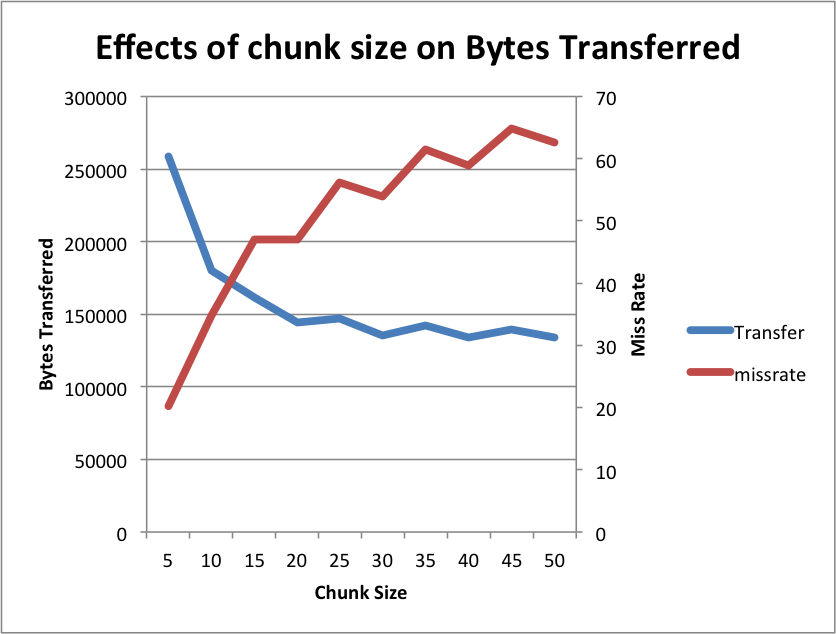
\includegraphics[scale=0.40]{images/chunksize2.png}
\caption{Effects of chunk size on Bytes Transferred. This graph takes into account the effects of the extra bytes that need to be transferred to account for the fingerprints that needs to be transferred to represent redndant chunks.}
\end{figure}

\begin{figure}[h] 
\centering 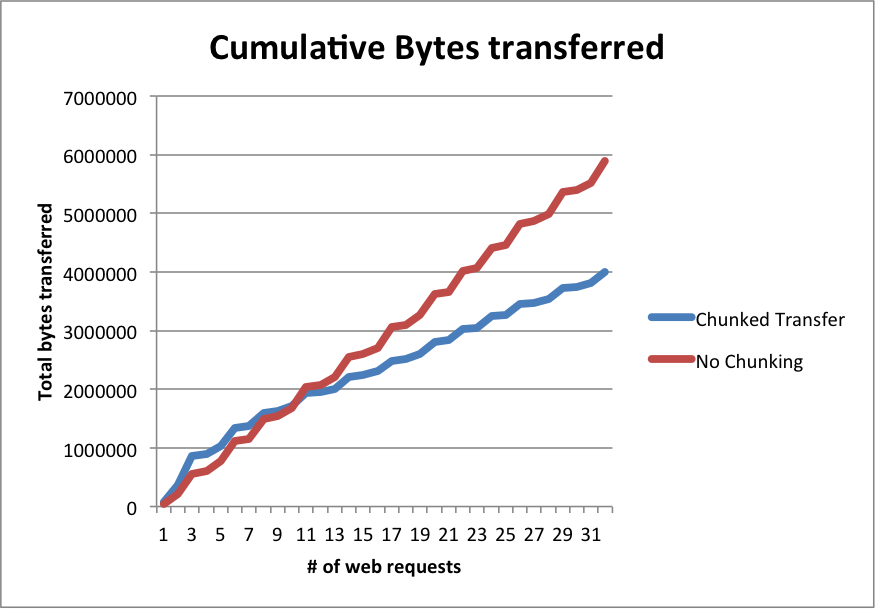
\includegraphics[scale=0.40]{images/cumulbrowsing.png}
\caption{Cumulative bytes transferred during browsing. This shows the bandwidth savings obtained from chunking.}
\end{figure}

\begin{figure}[h] 
\centering 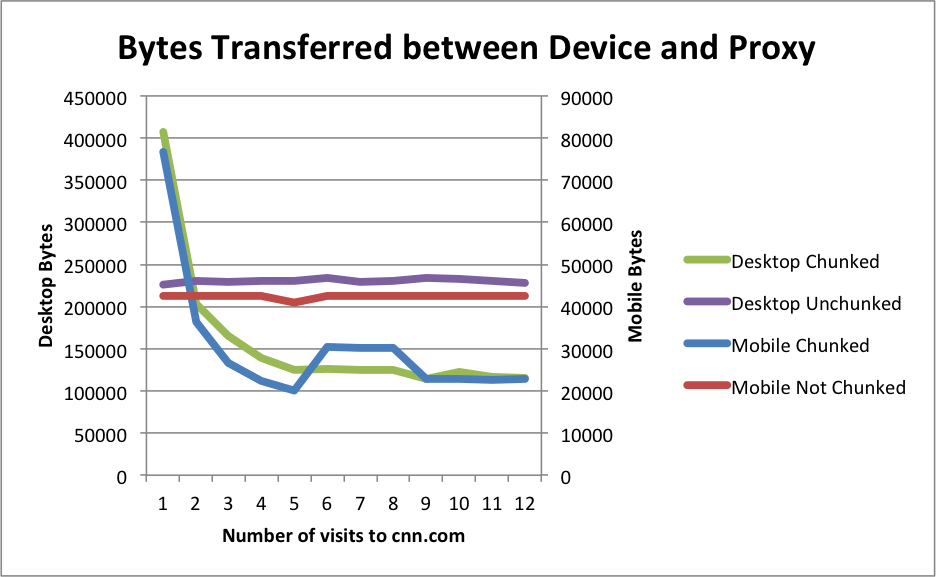
\includegraphics[scale=0.40]{images/desktopmobile.png}
\caption{Desktop vs Mobile Browser page differences.}
\end{figure}

\subsection{Different Cache Eviction Schemes}

\begin{figure}[h]
\centering 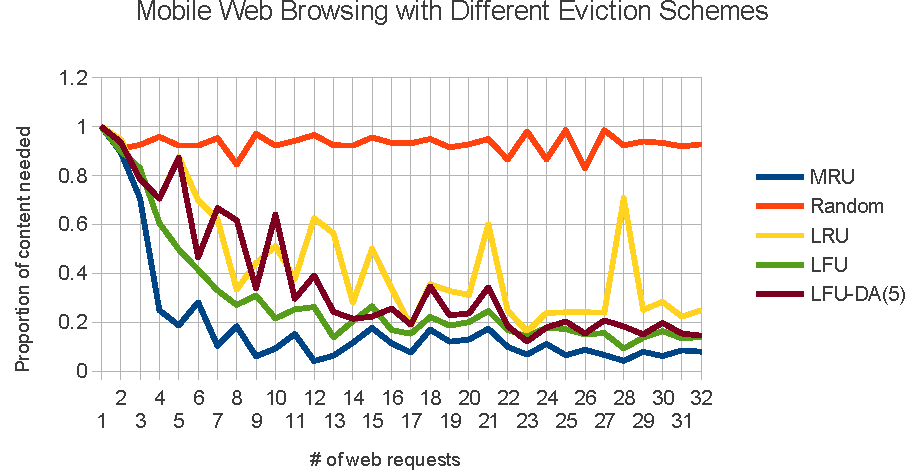
\includegraphics[scale=0.60]{images/caches.pdf}
\caption{Different Caches Performance}
\end{figure}